\documentclass[tikz,border=15pt]{standalone}
\usepackage{helvet}
\renewcommand{\familydefault}{\sfdefault}
\usepackage{tikz}
\usetikzlibrary{arrows.meta, positioning, fit, calc, shapes.geometric, automata}

\definecolor{emeraldpine}{HTML}{1A4D3E}
\definecolor{harvardcrimson}{HTML}{A51C30}
\definecolor{ethdarkblue}{HTML}{1F407A}
\definecolor{ethpetrol}{HTML}{007A87}
\definecolor{ethbronze}{HTML}{B87333}
\definecolor{ethpurple}{HTML}{5B4B8A}
\definecolor{ink}{HTML}{1A202C}
\definecolor{softink}{HTML}{4A5568}
\definecolor{paleink}{HTML}{A0AEC0}
\definecolor{cardbg}{HTML}{F8FAFC}
\definecolor{shadecolor}{HTML}{F4F6F9}

\begin{document}
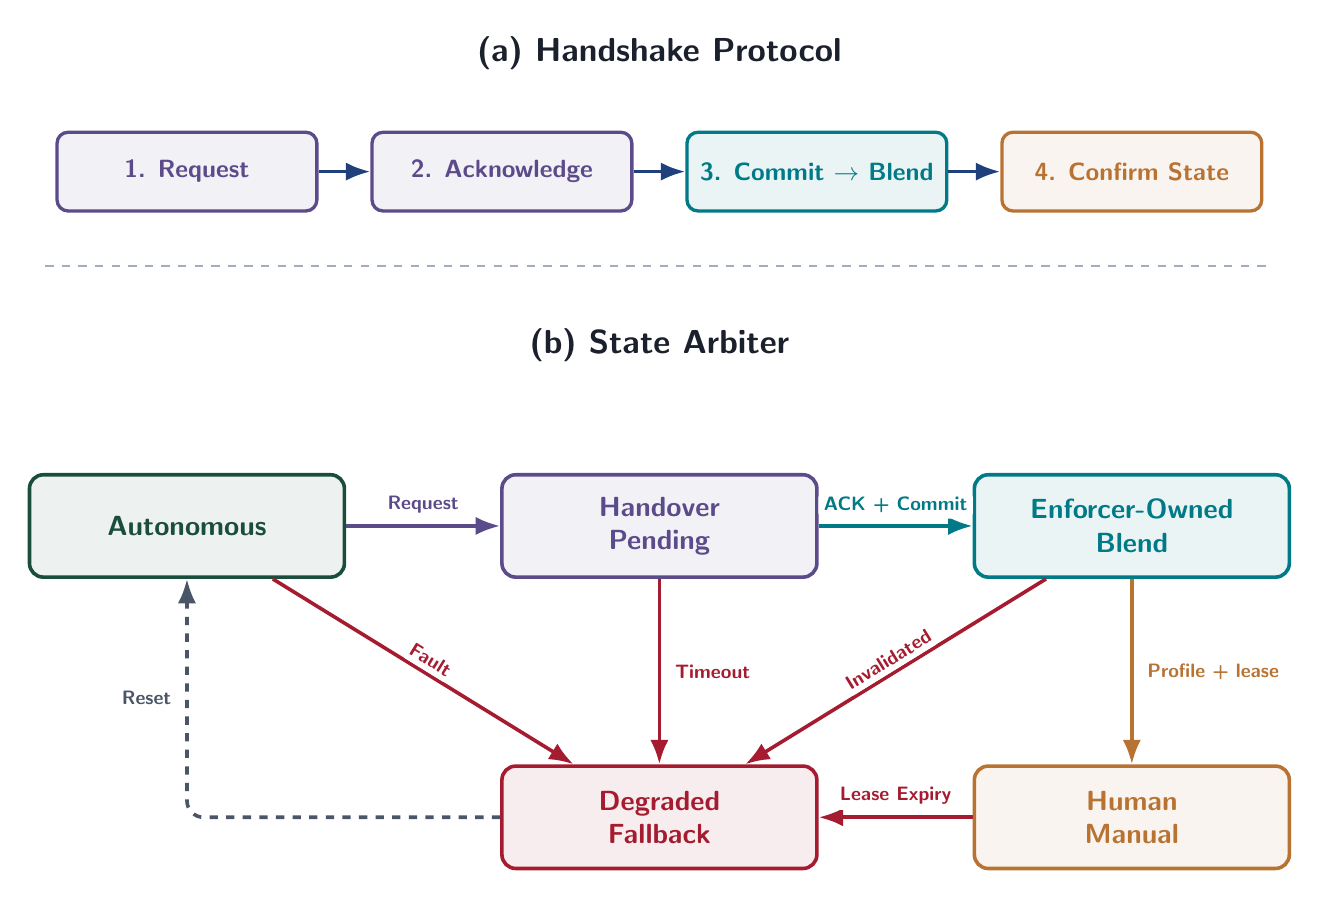
\begin{tikzpicture}[
    >=Latex,
    font=\sffamily,
    state/.style={
        rectangle, 
        rounded corners=5pt,
        draw=#1, 
        fill=#1!8, 
        line width=1.3pt,
        minimum width=4.0cm, 
        minimum height=1.3cm,
        align=center,
        text=#1,
        font=\sffamily\bfseries
    },
    proto/.style={
        rectangle, 
        rounded corners=4pt,
        draw=#1, 
        fill=#1!8, 
        line width=1.2pt,
        minimum width=3.3cm, 
        minimum height=1.0cm,
        align=center,
        text=#1,
        font=\sffamily\bfseries\small
    },
    arrow/.style={
        ->, 
        line width=1.3pt, 
        color=ethdarkblue,
        >=Latex
    },
    tlabel/.style={
        font=\sffamily\scriptsize\bfseries,
        text=#1,
        align=center,
        fill=white,
        inner sep=2pt,
        rounded corners=2pt
    }
]

% Panel (a)
\node[font=\sffamily\bfseries\large, text=ink] (panela) at (8, 2.5) {(a) Handshake Protocol};

\node[proto=ethpurple] (p1) at (2, 1) {1. Request};
\node[proto=ethpurple] (p2) at (6, 1) {2. Acknowledge};
\node[proto=ethpetrol] (p3) at (10, 1) {3. Commit $\rightarrow$ Blend};
\node[proto=ethbronze] (p4) at (14, 1) {4. Confirm State};

\draw[arrow] (p1) -- (p2);
\draw[arrow] (p2) -- (p3);
\draw[arrow] (p3) -- (p4);

% Divider
\draw[dashed, draw=paleink, line width=1pt] (0.2, -0.2) -- (15.8, -0.2);

% Panel (b)
\node[font=\sffamily\bfseries\large, text=ink] (panelb) at (8, -1.2) {(b) State Arbiter};

% States
\node[state=emeraldpine] (s1) at (2, -3.5) {Autonomous};
\node[state=ethpurple] (s2) at (8, -3.5) {Handover\\Pending};
\node[state=ethpetrol] (s3) at (14, -3.5) {Enforcer-Owned\\Blend};

\node[state=ethbronze] (s4) at (14, -7.2) {Human\\Manual};
\node[state=harvardcrimson] (s5) at (8, -7.2) {Degraded\\Fallback};

% Transitions
% s1 -> s2
\draw[arrow, draw=ethpurple] (s1) -- node[above=2pt, tlabel=ethpurple] {Request} (s2);

% s2 -> s3
\draw[arrow, draw=ethpetrol] (s2) -- node[above=2pt, tlabel=ethpetrol] {ACK + Commit} (s3);

% s3 -> s4
\draw[arrow, draw=ethbronze] (s3) -- node[right=3pt, tlabel=ethbronze] {Profile + lease} (s4);

% s2 -> s5
\draw[arrow, draw=harvardcrimson] (s2) -- node[right=3pt, tlabel=harvardcrimson] {Timeout} (s5);

% s3 -> s5
\draw[arrow, draw=harvardcrimson] (s3) -- node[sloped, above, tlabel=harvardcrimson] {Invalidated} (s5);

% s4 -> s5
\draw[arrow, draw=harvardcrimson] (s4) -- node[above=2pt, tlabel=harvardcrimson] {Lease Expiry} (s5);

% s1 -> s5
\draw[arrow, draw=harvardcrimson] (s1) -- node[sloped, above, tlabel=harvardcrimson] {Fault} (s5);

% s5 -> s1
\draw[->, line width=1.3pt, dashed, draw=softink, >=Latex, rounded corners=6pt] 
    (s5.west) -| node[pos=0.75, left=3pt, tlabel=softink] {Reset} (s1.south);

\end{tikzpicture}
\end{document}
